\documentclass[12pt,twoside]{article}
\usepackage[dvipsnames]{xcolor}
\usepackage{tikz,graphicx,amsmath,amsfonts,amscd,amssymb,bm,cite,epsfig,epsf,url}
\usepackage[hang,flushmargin]{footmisc}
\usepackage[colorlinks=true,urlcolor=blue,citecolor=blue]{hyperref}
\usepackage{amsthm,multirow,wasysym,appendix}
\usepackage{array,subcaption} 
% \usepackage[small,bf]{caption}
\usepackage{bbm}
\usepackage{pgfplots}
\usetikzlibrary{spy}
\usepgfplotslibrary{external}
\usepgfplotslibrary{fillbetween}
\usetikzlibrary{arrows,automata}
\usepackage{thmtools}
\usepackage{blkarray} 
\usepackage{textcomp}
\usepackage[left=0.8in,right=1.0in,top=1.0in,bottom=1.0in]{geometry}
\usepackage{pdfpages}
\newcommand*{\defeq}{\stackrel{\text{def}}{=}}
\newcommand{\R}{\mathbb{R}}
\newcommand{\rank}{rank}
\newcommand{\Tr}{Trace}
\newcommand{\sT}{T}
\title{Linear Algebra HW 10}
\author{gjd9961 }
\date{November 2021}


\begin{document}

\maketitle

\newpage

\section{Problem 10.1}
Let $A \in \R^{n \times m}$ and $y \in \R^n$, we consider the least squares problem as minimize $||Ax - y || ^2 $ with respect to $x \in \R^m$. \\

a) Show that $x^{LS} \perp Ker(A)$ \\

To show this property, we can leverage a couple pieces of information that we have from lecture, as well as proofs from past homeworks. We know from our work with SVD that any matrix $A \in \R^{n\times m}$ can be represented as $A = U\Sigma V^T$, and that the first $r$ columns of $U$ will form the basis of the Image of $A$, where the $Rank(A) = r$, and that the first $r$ columns of $V$ will define the basis of the row space, and the columns $V_{r+1}, \dots, V_{m-r}$ will define the basis of the Kernel of A. We also know the following that $A^{\dagger} = V\Sigma ' U^T$. 


By definition, $x^{LS}$ is a vector in the input space, $\R^m$,  and thus will be some linear combination of $v_1, \dots, v_r$, that is the first $r$ columns of $V$. Becasue all of the columns of $V$ are orthonormal, it follows that the columns $v_{r+1}, \dots, v_{m-r}$ that form the basis of $Ker(A)$ are orthogonal to the first $r$ columns of $V$, so $v_1, \dots, v_r \perp v_{r+1}, \dots, v_{m-r}$ and thus $x^{LS} \perp Ker(A)$\\

b) Deduce that $x^{LS}$ is the solution that has the smallest Euclidian norm. \\ 

We know from lecture that we can take a solution for $x^{LS}$ and add some vector from the Kernel of A, that solution will still be a minimizer. We can express it with the following set notation:
$$
    \{A^{\dagger}y  + v  | v \in Ker(A) \}
$$
But since we are adding non-zero vectors and thus values to the minimizer solution, it's euclidean norm will grow. Lets define an alternative solution to our minimizer $x^{LS}$, and lets call it $x^{Alt}$ where $x^{ALT}$ is $A^{\dagger}y + v$ where $v \in Ker(A)$. 

\begin{equation}
    \begin{split}
        ||x^{LS}||^2 &< ||x^{Alt}||^2 \\ 
        ||A^{\dagger}y||^2 &< ||A^{\dagger}y + v ||^2 \\ 
        ||A^{\dagger}y||^2 &< ||A^{\dagger}y||^2 + 2\langle v, A^{\dagger}y \rangle + ||v ||^2 \\     
        ||A^{\dagger}y||^2 &< ||A^{\dagger}y||^2 + ||v ||^2 \text{ since } A^{\dagger}y \perp v \text{ by part (a)} 
    \end{split}
\end{equation}
Therefore, the minimizer with the smallest norm is $x^{LS}$.
 
 \newpage 
\section{Problem 10.2}
Let $A \in \R{n \times d}$ and $y\in \R^n$. The ridge regression adds a $l_2$ penalty to the least squares term. Minimize $||Ax-y||^2 + \lambda ||x||^2$ with respect to $x\in \R^d$ for some penalization parameter $\lambda > 0 $ \\ 

a) Without solving 2, show that 2 admits a unique solution. You can use HW 9 results, but justify everything you use. \\

We know from HW 9 that if you add a convex function to a convex function the result function is a convex function. So therefore, the function will have a minimizer. But we're not sure if this minimizer is unique.

Fortunately, we also know from HW 9 that if a matrix is Positive Definite, then it is strictly convex, and admits a unique minimizer. Furthermore, we know that we can make a matrix positive definite by making its eigenvalues positive definite. We also know from past home-works that we can add some $\lambda \times Id_n$ to a matrix $A$ where $\lambda >0$ and the result is the eigenvalues of $A$ get increased by $\lambda$. When we play around with the equation in part b, we will show how the ridge regression minimizer function is positive definite (and invertible) and thus will admit a unique solution. \\


b) Show that the solution is given by:
$$
x^{Ridge} = (A^TA + \lambda Id_n)^{-1} A^Ty 
$$
Justify your answer precisely including why $(A^TA + \lambda Id_n)^{-1}$ exists. \\

So here what we want to do is take the gradient of the original minizer function, and set it to 0. Then well get our expression, and we can elaborate why $(A^TA + \lambda Id_n)^{-1}$ exists. 

\begin{equation}
    \begin{split}
        f(x) &= ||Ax-y||^2 + \lambda ||x||^2 \\
        \nabla f(x) &= A^T(Ax -y) +\lambda x  \text{ using the properties from lec/hw 9} \\
        \nabla f(x) = 0 &= A^TAx - A^Ty  + \lambda x \text{ set the gradient to 0 and solve for x} \\
        A^TAx + \lambda x &= A^Ty  \\
        (A^TA+\lambda Id_n)x &= A^Ty \qed
    \end{split}    
\end{equation}
Like we said in part a) we know that for some choice of $\lambda >0$ we can make $A^TA$ positive definite and therefore, strictly convex and invertible (which is why $(A^TA + \lambda Id_n)^{-1}$ exists).  Therefore, for some $\lambda$ we have: 
$$
x^{ridge} = (A^TA + \lambda Id_n)^{-1}A^Ty
$$
 \newpage 
\section{Problem 10.3}
Recall that $||M||_{sp}$ denotes the spectral norm of a matrix $M$. \\
a) Let $A \in \R^{n\times m}$. Show that for all $x \in \R^m$:
$$
    ||Ax|| \leq ||A||_{sp}||x|| 
$$ \\

To solve this we're going to have to reexpress some of the terms in our inequality. Firstly, $||Ax|| = \sqrt{x^TA^TAx}$ We can evaluate this expression further as we know a few properties of the $A^TA$ term in the middle. Firstly, that $A = U\Sigma V^T$:
$$
    A^TA = V\Sigma ^T U^T U \Sigma V^T = V\Sigma ^2 V^T
$$
Where $\Sigma$ is the squared eigenvalues of $A^TA$, and $U,V^T$ are orthogonal matrices. And, since we know that $x \in \R^m$ and $V \in \R^{m \times m}$ and $V$ is orthonormal, we can express $x$ in terms of $V$.
$$
x = \sum_{i=1}^{min(n,m)} \alpha_i v_i
$$
where $\alpha \in \R$ and $v_1, \dots, v_m$ are the orthonormal columns of $V$. So what we now have is:
\begin{equation}
    \begin{split}
          ||Ax||^2 = x^TA^TAx &= \sum_{i=1}^{min(n,m)} \alpha_i v_i^T \times A^TA \sum_{i=1}^{min(n,m)} \alpha_i v_i \\
          ||Ax||^2 &= \sum_{i=1}^{min(n,m)} \alpha_i v_i^T \times (\sum_{i=1}^{min(n,m)} \alpha_i (A^TAv_i)) \\
          ||Ax||^2 &= \sum_{i=1}^{min(n,m)} \alpha_i v_i^T \times (\sum_{i=1}^{min(n,m)} \alpha_i (\lambda_i v_i)) \\
          ||Ax||^2 &= c_i^2 \lambda_i u_i^Tu_i = c_i^2 \lambda_i 
    \end{split}
\end{equation}
Therefore, the upper bound of the transformation $||Ax||^2$ and thus $||Ax||$ is constrained by the largest Eigenvalue of $||Ax||$ hence the connection to the spectral norm of $A$. Therefore, we have:

$$
    ||Ax|| \leq \sqrt{\lambda_{max} \sum_{i=1}^{min(n,m)} c_i^2} = ||A||_{sp} || x|| \qed
$$




b) Show that for all $A \in \R^{n \times m}$ and $B \in \R^{m\times k}$: 
$$
  ||AB||_{sp} \leq ||A||_{sp}||B||_{sp}
$$

we can use a little trick with a vector with norm 1 to show this property, and with using what we saw in part a. Let $y \in \R^k$ and $||y|| = 1$, therefore:

$$
    ||ABy|| \leq ||A||_{sp} ||By|| \leq ||A||_{sp} ||B||_{sp}||y|| = ||A||_{sp} ||B||_{sp} 
$$
We know that to maximize $||ABy||$ we'd have to set $||y||=1$ which is the definition of the spectral norm of $||AB||$ so therefore:
$$
    ||AB||_{sp} \leq ||A||_{sp}||B||_{sp} \qed
$$


\section{Problem 10.4}
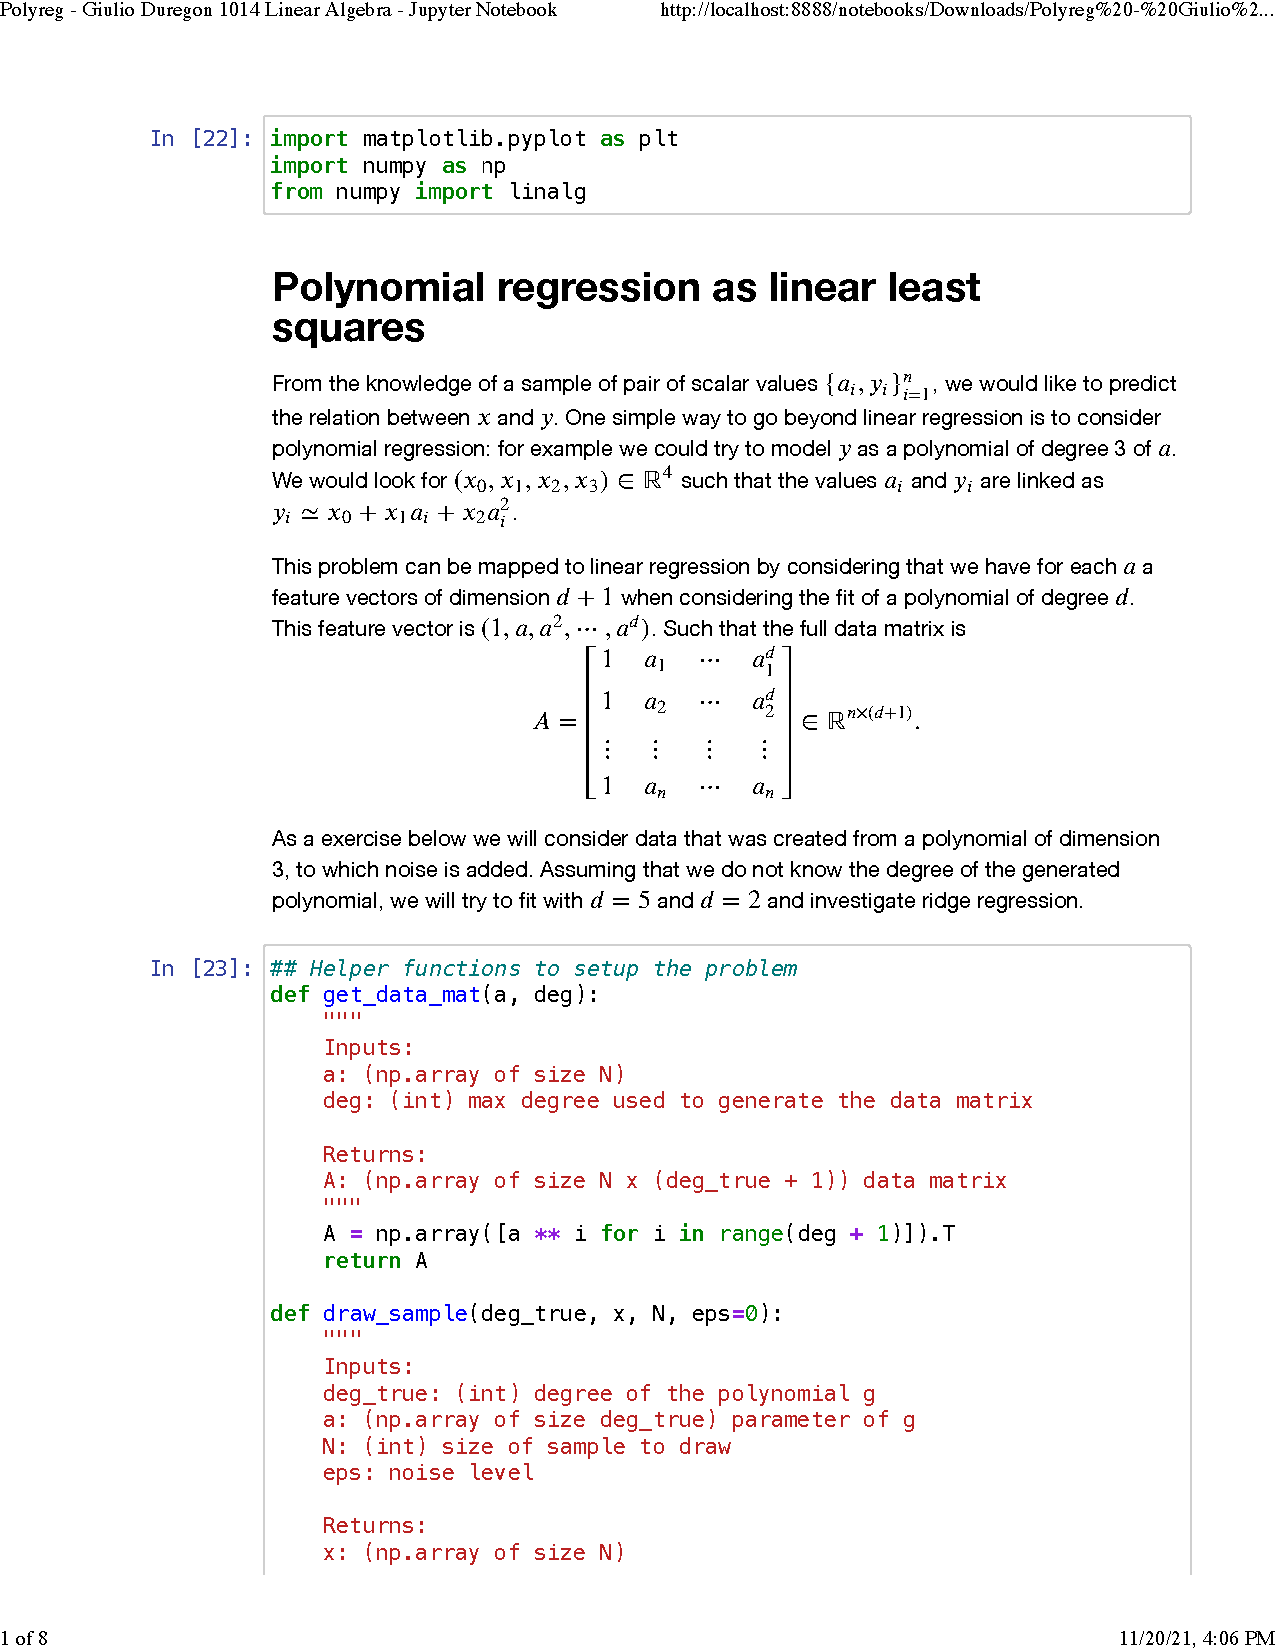
\includepdf[pages=-]{code.pdf}



\end{document}